\documentclass[11pt, a4paper, DIV=12]{scrartcl}

% useful packages 
\usepackage{mathtools}
\usepackage{physics}
\usepackage{graphicx}					  
\graphicspath{{figs/}}



\usepackage{amssymb}
\usepackage{amsmath}
\usepackage{hyperref}
\usepackage[separate-uncertainty=true]{siunitx}
\usepackage{xcolor}
\usepackage{braket} % easy braket notation
\usepackage{enumitem}
\usepackage{booktabs}
\usepackage{here}
\usepackage{cprotect}

\usepackage[backend=biber, sorting=none]{biblatex}
\bibliography{refs.bib}

% \numberwithin{equation}{section}

\title{Simulation of 1-Dimensional Ising Model}
\date{\today}
\author{Harilal Bhattarai \& Marcel Schindler}
\begin{document}
	\maketitle
	
\section{Introduction}
The Ising model is a wonderful sandbox to study critical phenomena with numerical methods. It helps to investigate the magnetization in the absence of the external magnetic field.\\

In this report, firstly, We can include some theoretical background on theory part. Secondly, we will try to present the answers the questions of this exercise-sheet-1 in analysis part, also, with illustration of the results of simulation with the help of plots.  

\section{Theory}

This system of spins is immersed in a heat bath of constant temperature T and in an external magnetic field h. Its dynamics are governed by the Hamiltonian,
\begin{equation}
H(s)= -J \sum_{<x,y>}s_{x}s_{y} - h \sum_{x}s_{x}
\end{equation}
$ <x,y> $ denotes the nearest-neighbor pair x and y on the chain, J is a real number and we assume periodic boundary conditions. That means that spins couple only to the nearest neighbor and $s_{N-1}$ couples with $s_0$ with N the number of total spin-particles. We define the partition function:
\begin{equation}
	Z= \sum_{s'} \exp(-\frac{H(s')}{k_B T})
\end{equation}
where we sum over all possible spin field $s=(s_0,s_1,...,s_{N-1})$. For simpler notation, we switch the system of units such that $k_B=1$. We this assumption we get the dimensionless ratios $\frac{J}{T}$ and $\frac{h}{T}$.

In 1d the partition function can be determined analytically as a function of N, J/T, and h/T as,
\begin{equation}
\text{Z}=\lambda^{\text{N}}_{+} + \lambda^{\text{N}}_{-}
\end{equation}
Where, 
\begin{equation}
 \lambda^{\text{N}}_{\pm}= e^{\frac{J}{T}} \bigg(cosh(\frac{h}{T})\pm \sqrt{Sinh(\frac{h}{T})^2 + e^{-4(\frac{J}{T})}} \bigg) 
 \label{Equ:lambda}
	\end{equation}
The magnetization can be determine with the help of Ising model as, 
\begin{equation}
<m> = \frac{\text{h}}{\text{T}} \frac{\partial\log \text{Z}}{\partial \text{h}}
\label{equ:m}
\end{equation}  

\section{Analysis}
In the partition function J is the coupling constant between two spins. We assume only direct neighbors have $J\neq 0$. For $J>0$ we call the interaction ferromagnetic. With other words, the spins tend to align parallel to the external Magnetic field. Ferromagnetic materials will form permanent magnets. For $J<0$ we call the interaction antiferromagnetic. So the spins are antiparallel and we dont get any permanent magnitization.\\

To determine the dependency of $ <m> $ on the external field strength h for fixed N and the number of spins N for fixed h. To do so, we have taken the N=20, J=1 and $h \in [-1, 1]$. Here, for analytic solution we used the expression \ref{equ:m}.

To compare these both(numeric and analytic) results, we plotted a graph numbers vs magnetization with change the external magnetic field. From figure \ref{fig:Nconst}, we can see that the magnetization is linear in h. In other words the magnetization depends linear with the external magnetic field. We would expect to have no magnetization with no external magnetic field and we see this is the case for h=0. Also we can see that the numeric and analytic solution match perfectly.
\begin{figure}[H]
	\centering
	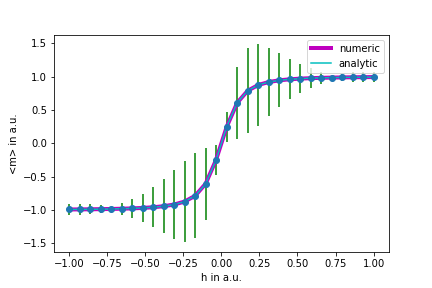
\includegraphics[width=0.8\linewidth]{Nconst.png}
	\caption{The number of spins N for fixed h.}
	\label{fig:Nconst}
\end{figure}


Again, we have plotted a graph number vs magnetization with considering constant external magnetic field. We have chosen $h= 0.5$. From figure \ref{fig:hconst} we can see that change N but since we are looking for the magnetization per spin. We expect that it does not change with higher N and this is the case. In this plot we see that the numerical and analytical solution don't match perfectly but the presicion is still very good. 
   \begin{figure}[H]
   	\centering
   	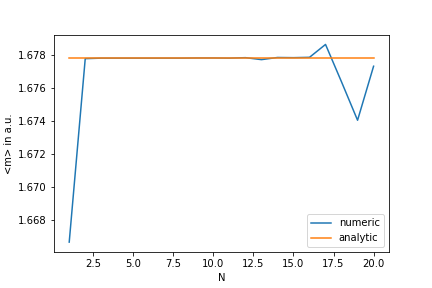
\includegraphics[width=0.8\linewidth]{hconst.png}
   	\caption{The external field strength h for fixed N.}
   	\label{fig:hconst}
   \end{figure}
\section{conclusion}
In conclusion, on the basis of above analytic and numerical analysis of the system, we conclude that in the ferromagnetic materials the internal magnetic field is parallel to the external field. Since, they are linearly interrelated. Also, we claim that these both methods match each other quite good and give the solution to the given problem. And, another interesting result, we saw that the magnetization per Spin does not change with more particles.  
\begin{thebibliography}{12}
\bibitem{exercise-sheet} 
	Thomas Luu, Andreas Nogga, Marcus Petschlies and  Andreas Wirzba, Exercise-sheet, 2020. 
		
\bibitem{wiki} 
	Satya pal singh, \textit{The Ising Model: Brief Introduction and Its Application}, 2020.
	
\end{thebibliography}

\end{document}
